%%% Local Variables:
%%% TeX-engine: xetex
%%% End:

% Deadlines - 23.

\documentclass[12pt]{article}
\usepackage{geometry}
\usepackage{textcomp}
\usepackage{gensymb} %grādu simbols
%\usepackage[utf8]{inputenc}
\usepackage{tcolorbox}
\usepackage{multicol}
\usepackage{enumitem}
\usepackage{indentfirst}
\usepackage[bf,center]{titlesec} %izveido atstarpes starp chapter un section nosaukumu
\usepackage{tocloft}
\usepackage{hyperref}
\usepackage{tabularx}
\usepackage{ragged2e}
\usepackage{tocloft}
\usepackage{secdot}
\usepackage{amsmath}
\usepackage{placeins}

\newcommand{\fakesection}[1]{%
  \par\refstepcounter{section}% Increase section counter
  \sectionmark{#1}% Add section mark (header)
  \addcontentsline{toc}{section}{\protect\numberline{\thesection}#1}% Add section to ToC
  % Add more content here, if needed.
}

\newcommand{\komentars}[1]{}


\usepackage[citestyle=authoryear,bibstyle=nature,uniquename=false]{biblatex}

\addbibresource{bibliografija.bib}
\renewcommand*{\nameyeardelim}{\addcomma\space}

\usepackage{csquotes}



%latviešu val. lokalizācija
\usepackage[latvian,english]{babel}
\addto\captionslatvian{\renewcommand{\figurename}{attēls}\renewcommand{\tablename}{tabula}}

\usepackage{titlesec}%izveido atstarpes starp chapter un section nosaukumu
\titleformat{\chapter}
  {\normalfont\fontsize{16}{18}\bfseries\raggedright}{\thechapter.}{0pt}{\MakeUppercase}{}
  
\titleformat{\section}
  {\normalfont\fontsize{14}{16}\bfseries}{\thesection}{1em}{}
\titleformat{\subsection}
  {\normalfont\fontsize{12}{16}\bfseries}{\thesubsection}{1em}{}  

\titlespacing*{\chapter}{0pt}{0pt}{10pt}
\titlespacing*{\section}{0pt}{5pt}{5pt}

\usepackage[labelfont={bf}]{caption}%attēlu un tabulu nosaukumu fonts



%fontam
\usepackage[no-math]{fontspec}

\setmainfont{Times New Roman}



%\hypersetup{
%	colorlinks=true,
%	linkcolor=black,  
%	urlcolor=blue
%}

\urlstyle{rm}

\titlespacing*{\section}{0pt}{0pt}{1.5pt}
\titlespacing*{\subsection}{0pt}{0.5\baselineskip}{1.5pt}
\titlespacing*{\subsubsection}{0pt}{0.5\baselineskip}{1.5pt}
\titleformat{\section}{\large \bfseries \centering}{\thesection}{1em}{}%section formatting
\titleformat{\subsection}{\normalsize \bfseries
	\centering}{\thesubsection}{1em}{}%subsection formatting
\titleformat{\subsubsection}{\normalsize \bfseries
	\centering}{\thesubsubsection}{1em}{}%subsubsection formatting
\geometry{a4paper, left=2.5cm, right=2.5cm, top=2.5cm, bottom=2.5cm}

\linespread{1.3}
\setlength{\parindent}{1cm}
\setlength{\parskip}{0pt}



\begin{document}
\selectlanguage{latvian} 
	\begin{titlepage}
		\begin{center}
			\vspace*{0.5cm}
			\begin{large}{Siguldas Valsts ģimnāzija}
                \vfill
                \textbf{No atmosfēriskā radio trokšņa iegūto gadījumskaitļu kvalitāte atkarībā no radio frekvences}
                \\Zinātniski pētnieciskais darbs fizikas nodaļā
                \vfill
				
			\end{large}
		\end{center}
		\vspace{3cm}
	
        {\raggedleft
        \begin{tabular}{l@{}}
        Darba autors: Atis Dubrovskis\\
        Darba vadītājs: Jānis Bukins\\
        \end{tabular}\par}\
		\vspace{3cm}
		\begin{center}
			Sigulda 2024
		\end{center}
	\end{titlepage}

    \addcontentsline{toc}{section}{Anotācija}
    \begin{abstract}
    Zinātniski pētnieciskā darba tēma ir \textbf{"No atmosfēriskā radio trokšņa iegūto gadījumskaitļu kvalitāte atkarībā no radio frekvences"}. 
    Darba autors: Atis Dubrovskis, Siguldas Valsts ģimnāzijas 11. klases skolnieks. Darba vadītājs:
    Jānis Bukins, Siguldas Valsts ģimnāzijas fizikas skolotājs. 
    Darbā tika izpētīta no atmosfēriskā radio trokšņa ģenerētu skaitļu, ar izveidotu programmu, statistiskā nejaušuma  kvalitāte atkarībā no atmosfēriskā radio trokšņa frekvences.
    Pētāmā problēma: \textbf{Kā no atmosfēriskā radio trokšņa ģenerētu nejaušu skaitļu kvalitāti ietekmēs izmantotā frekvenci, pie kuras ierakstīts atmosfēriskai radio troksnis?} \\
        Darbā gaitā tika secināts, ka:
\begin{itemize}
\Centering
        \item Pētijumā piedāvātais īstu gadījumskaitļu ģenerators statistiskajos pārbaudījumos uzstāda labākus rezultātus par bieži izmantoto Xorshift gadījumskaitļu ģeneratoru.
        \item Izmantojot radio frekvences, kurās iespējama makslīgo radio signālu iejaukšanās, ģenerēto skaitļu virkņu statistiskā nejaušuma kvalitāte būtiski samazinās.
        \item Balstoties uz pētijumu, iespējams mājās apstākļos iegūt pilnīgi nejaušus skaitļus no atmosfēriskā radio trokšņa.
\end{itemize}
Zinātniski pētnieciskais darbs sastāv no titullapas, ievada, galvenās daļas, kurā ietilpst 3
nodaļas, secinājumiem, izmantotās literatūras un avotu saraksta.
    \end{abstract}
    \selectlanguage{english} 
    \begin{abstract}
    The theme of scientific research is \textbf{“Quality of random numbers derived from atmospheric radio noise based on radio frequency”}
Author of the work: Atis Dubrovskis, 11th grade student of Sigulda State Gymnasium. Supervisor:
Jānis Bukins, a teacher of physics at Sigulda State Gymnasium.
The work explored the statistical randomness quality of numbers generated from atmospheric radio noise, with an established random number generation program, depending on the frequency of atmospheric radio noise. 
Research issue: \textbf {How will the quality of random numbers generated from atmospheric radio noise be affected by the frequency used at which atmospheric radio noise is recorded?}\\
The work concluded that:
\begin {itemize}
\Centering

\item the true random number generator proposed in the study sets better results than the often used Xorshift random number generator in statistical tests.

\item the statistical randomness quality of the generated numbers decreases significantly when using radio frequencies in which interference from artificial radio signals is likely.

\item it is possible to generate true random numbers from atmospheric radio noise at home.

\end {itemize}

Scientific research consists of a cover page, an introduction, a key part comprising of 3
chapters, conclusions, the literature used, and a list of sources.
    
    
    
    
    \end{abstract}
    \selectlanguage{latvian}
    
    \newpage
	\tableofcontents
    

    
	\pagebreak
    
	\section{Ievads}
    \addcontentsline{toc}{section}{Ievads}
    
	   Mūsdienās pastāv vajadzība pēc nejaušiem skaitļiem vairākās jomās: kriptogrāfijā, Montekarlo kalkulācijās, dažādās simulācijās.
       Mūsdienās viskritiskāk tie ir nepieciešami tieši kriptogrāfijā un tās daudzveidīgajos risinājumos un pielietojumos ikdienas dzīvē:
       bankomātos, e-komercijā, datu drošā uzglabāšanā un sūtīšanā, kā arī vispārīgi kiberdrošībā.
       Bet tikai ar standarta datora palīdzību nav iespējams tos iegūt ar augstu kvalitāti un neparedzamības rādītājiem, jo datori strādā  
       \textbf{determiniskti} un bez papildu aprīkojuma spēj ģenerēt gadījumskaitļus tikai ar pseido-gadījumskaitļu ģeneratoriem, kas nav \textbf{īsti nejauši} tādēļ pastāv nepieciešamība pēc īstu gadījumskaitļu ģeneratoriem un metodēm, kā nejaušus skaitļus iegūt ar pēc iespējas augstāku nejaušumu un kvalitāti, lai nodrošinātu augstāko iespējamo drošību un datu analīzes kvalitāti simulācijās un Montekarlo eksperimentos. 
       Pastāv dažādas metodes kvalitatīvu \textbf{patiesu nejaušu skaitļu} (TRN) ieguvei, bet visas balstās uz nejaušām fiziskām parādībām,  
       ko \parencite{patiesinejausie}
       %Štipčević \& Koç (2014) 
       iedala 4 grupās: 
       \begin{itemize}
            \item Haosa
            \item Džonsona trokšņa (termālā trokšņa)
            \item Zīnera trokšņa (elektriskā trokšņa)
            \item Radioaktīvās sadalīšanās
       \end{itemize} 
       Šajā darbā tiks aplūkota nejaušu skaitļu ieguve no atmosfēriskā radio trokšņa, kas iedalīts zem haosa parādībām, un tiks salīdzinātas un testētas dažādas frekvences, lai uzzinātu, kuras no tām rada kvalitatīvākos nejaušos skaitļus un uzrāda augstāko \textbf{entropiju}.    
       \textbf{Darba tēma:} no atmosfēriskā radio trokšņa iegūto gadījumskaitļu kvalitāte atkarībā no radio frekvences.\\
       \textbf{Darba mērķis:} noskaidrot, kā atmosfēriskā radio trokšņa frekvence ietekmē iegūto gadījumskaitļu kvalitāti.
       \\
       \textbf{Darba uzdevumi:} 
       \begin{enumerate}
           \item Izpētīt atmosfēriskā radio troksni un tā rašanos.
           \item Izveidot programmu, kas spēj no atmosfēriskā radio trokšņa uzģenerēt nejaušus skaitļus.
           \item Veikt nejaušo skaitļu analīzi izmantojot NIST nejaušo skaitļu eksperimentus un testus.
           \item Veikt datu analīzi.
       \end{enumerate}
       \textbf{Pētāmā problēma:} kā atmosfēriskā radio trokšņa frekvence ietekmē no tā ģenerēto nejaušo skaitļu kvalitāti.
       \textbf{Darba struktūra:} darbs sastāv no ievada, 3 nodaļām, 13 apakšnodaļām, secinājumiem, 26 izmantotās literatūras un informācijas avotiem. Darbā ir 2 attēli, 8 tabulas, 2 pielikumi.
       
       
       
	
	\pagebreak
	\section{Literatūras apskats}
	%\addcontentsline{toc}{section}{Literatūras apskats}
    % Nejaušo skaitļu ģenerēšana izmantojot atmosfērisko troksni
    % Atmosfēriskais troksnis
    % Haotiskas dabas pārādības
    % Haosa teorija
    %\subsection{Elektromagnētiskie viļņi}
    %Elektromagnētiskie viļņi ir 
    
    %Pie mazākām frekvencēm vairāk rada zibens izlādes, grafiks, kas to attēlo.
    %Ko darīt:
    % 3 ieraksti un dati ar vnk skaņu
    % 3 ieraksti un dati ar korg ms 20minis
    %\pagebreak
   
    \subsection{Atmosfēriskais radio troksnis}
    Atmosfēriskais radio troksnis ir radio troksnis, ko pārsvarā rada zibens elektriskās izlādes, globālā mērogā notiek aptuveni $44 (\pm $5) zibens izlādes sekundē \parencite{zibens}, un kosmiskais fona starojums. To  modelē kā ar Puasona saistītu procesu, kas balstās uz galvenajiem faktoriem: globālo zibens izlāžu sadalījumu, to izplatīšanos un kosmiskā starojuma troksni, kas atgādina balto troksni. \parencite{atmosf_modelis} 
    \par Atmosfēriskais radio troksnis, kas sastāv no fona elektromagnētiskā trokšņa, parasti ir spēcīgāks par paša radio uztvērēja radīto troksni frekvencēs līdz 20 MHz, kā arī atmosfērisko troksni pilsētvidē traucē mākslīgie elektromagnētiskā trokšņa avoti, tādēļ "viskvalitatīvāko", jeb entropijas bagātāko troksni var iegūt ārpus tām, kur pastāv minimāls mākslīgais elektromagnētiskais troksnis. \parencite{atdalisanas}
    Atmosfēriskais radio troksnis, ko rada tālu spēcīgu zibens elektrisko izlāžu impulsa troksnis pārsvarā izplatās caur \textbf{zemes viļņiem} \parencite{zibens2}, kā arī jonosfēras refrakcijas, savukārt kosmiskais fona radio troksnis izplatās caur jonosfēras diafragmu, kas ir apļveida lauks jonosfērā, kas ir caurspīdīgs elektromagnētiskajam troksnim atkarībā no frekvences, ar ko tiek uztverts radio troksnis un jonosfēras plazmas frekvences virsotnes. \parencite{zibens3} 

    
    \begin{figure}[!ht]
    \centering
    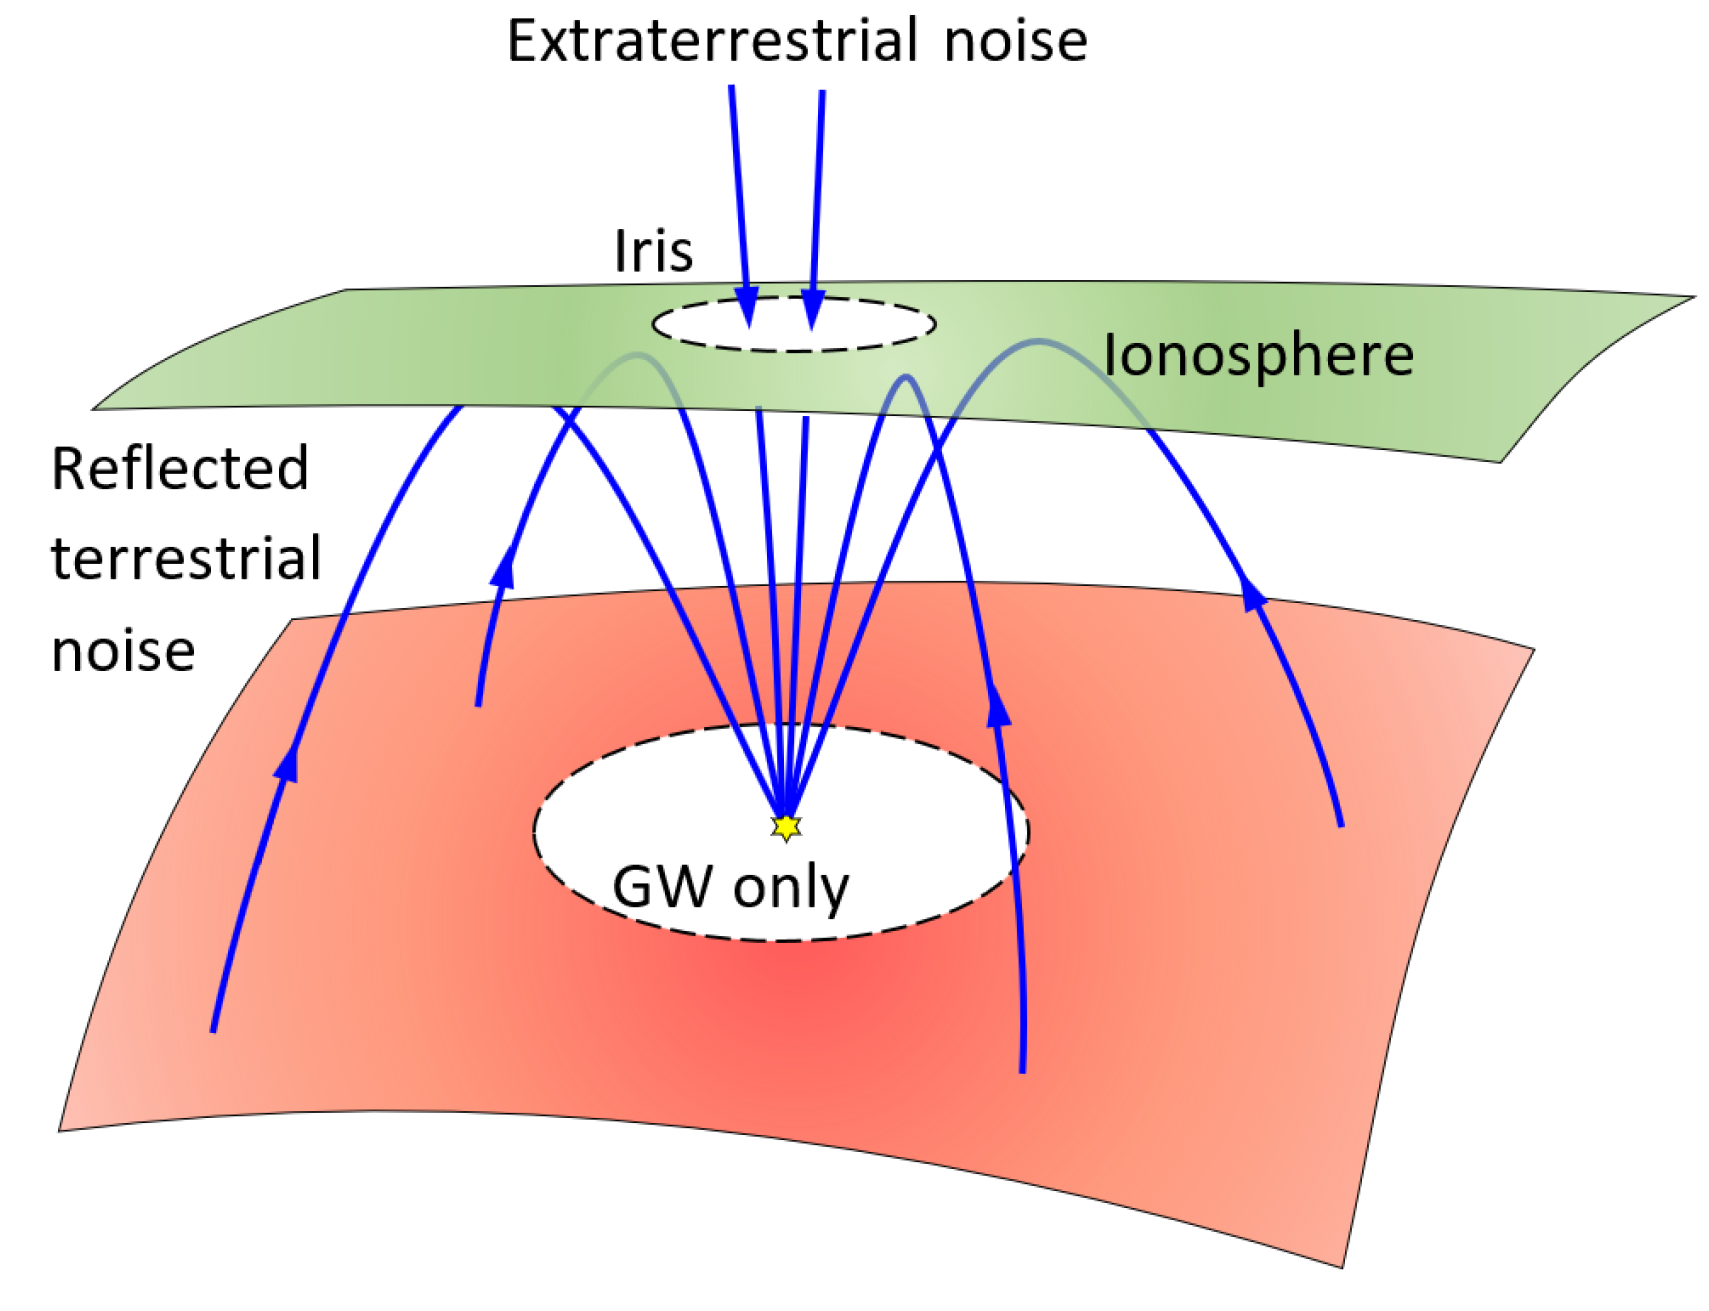
\includegraphics[width=0.5\textwidth]{attēli/zimejums.png}
    \caption{Atmosfēriskā radio trokšņa veidojošā zemes fona trokšņa un kosmiskā fona trokšņa izplatība uz radio uztvērēju. \parencite{atdalisanas}}
    \label{fig:zimejums}
\end{figure}
     Atmosfērisko radio troksni var raksturot kā \textbf{deterministisku} parādību, tāpēc teorētiski, ja ir pietiekamas zināšanas par atmosfēras procesiem, šo radio troksni ir iespējams paredzēt, bet tas ir nereālistiski, jo būtu nepieciešams zināt katras atmosfēras molekulas pozīciju un paātrinājumu, tāpēc var šo parādību raksturot kā nejaušu, lielā skaita nezināmu mainīgo dēļ. \parencite{randomorg}. Atmosfērisko radio troksni var uzskatīt par nejaušu, atmosfēras milzīgā izmēra un tajā dabiski notiekošo sīko izmaiņu dēļ. \parencite{troksnisirrandom} Šīs sīkās izmaiņas norisinās konstanti, kā arī, ņemot vērā augsto zibens elektrisko izlāžu ietekmi uz atmosfērisko troksni un zibens izlāžu lielo elektromagnētisko dažādību un neparedzamību \parencite{zibensneparedzamiiba}, šo procesu var skaidrot kā haotisku un nejaušu.
    
    \subsection{Gadījumskaitļu ģeneratori}
    Mūsdienu pasaulē arvien vairāk tiek izmantoti dažādi digitāli risinājumi, kam ir nepieciešamība pēc drošas datu šifrēšanas, piemēram, tiešsaistes banku sistēmās, drošiem darījumiem \parencite{new_century_generation}, kā arī stohastiskajā modelēšanā un īpaši svarīga ir šo gadījumskaitļu \textbf{turpmāk - nejaušu skaitļu} ģeneratoru kvalitāte, lai skaitļi būtu pēc iespējas neparedzamāki, tādējādi nodrošinot augstu drošības pakāpi un izvairoties no kļūdainiem rezultātiem stohastiskajos modeļos un \textit{Montekarlo} eksperimentos. \parencite{notsoeasytofind}
    Lai iegūtu nejaušus skaitļus, ir nepieciešamība pēc kvalitatīviem gadījumskaitļu, jeb nejaušu skaitļu ģeneratoriem, kas pēc kāda noteikta algoritma spēj ģenerēt nejaušus skaitļus. Pastāv dažādi nejaušu skaitļu ģeneratoru veidi: \emph{pseido-nejaušu skaitļu ģeneratori} (PNSĢ) un \emph{īsti nejauši skaitļu ģeneratori} (ĪNSĢ).
    \par Pseudo-nejaušu skaitļu ģeneratori ir visizplatītākie nejaušu skaitļu ģeneratori; nejaušus skaitļus tie iegūst, apstrādājot noteiktus jau zināmus vai programmatūrā nosakāmus skaitļus pēc noteikta algoritma, izmantojot kā pamatu, jeb \textbf{sēklu} (seed) skaitļus, kas sastāv no dažādiem paredzamiem parametriem, piemēram, datorsistēmas laika mikrosekundēs. \parencite{pseudo} Šo PNSĢ galvenā priekšrocība ir, ka tie ir ļoti efektīvi, nepatērē daudz resursu un tiem nav nepieciešams papildu aprīkojums, taču šie PNSĢ nespēj sniegt 
    pietiekami kvalitatīvus nejaušus skaitļus, savukārt, jo datori strādā pēc noteiktiem algoritmiem un būtībā ir \textbf{deterministiski} \parencite{nist_ir_slikts}, tāpēc no PRNG nevar iegūt īsti nejaušus skaitļus un ir salīdzinoši viegli paredzami \parencite{pseudo}. Pastāv arī īsti nejaušu skaitļu ģeneratori (ĪNSĢ), kas skaitļus ģenerē no dažādām haotiskām, jeb nejaušām dabas parādībām, kuras nevar
    precīzi noteikt un paredzēt, radot augstu entropijas, jeb nejaušuma pakāpi.\parencite{patiesinejausie} Pastāv arī dažādi ĪNSĢ varianti, kas iedalās 4 galvenajās kategorijās:  no brīvgaitas oscilatoriem, no haotiskām parādībām, t. sk. radioaktīvās sadalīšanās \parencite{radioaktivais_troksnis}, no kvantu parādībām un no trokšņa: Džonsona, jeb  termālā trokšņa \parencite{dzonsona_troksnis}, Zēnera, jeb elektriskā trokšņa \parencite{elektriskais_troksnis}, un ar atmosfērisko troksni \parencite{patiesinejausie}, kas tika pētīts šajā pētījumā. Nejaušu skaitļu ģeneratori ir nepieciešami daudzās jomās,
    un ir jomas, kurās nav būtiska nepieciešamība pēc kvalitatīviem nejaušiem skaitļiem, un pietiek ar PNSĢ skaitļu
    ģeneratoriem arī tādēļ, ka tie ir daudz efektīvāki un patērē mazāk laika un resursu (sistēmas izmaksas utt.),
    \parencite{randomorg}, zemāk var apskatīt abus nejaušo skaitļu ģeneratoru tipus:
    
\begin{table}[!ht]
        \centering
       

\begin{tabular}{ |c|c|c| }% c automātiski padara kolonnu tik garu cik vajag
\hline
Īpašība & \textbf{Pseido-nejaušu skaitļu ģeneratori} & \textbf{Īsti nejaušu skaitļu ģeneratori}  \\
\hline
Efektivitāte & Izcila & Vāja\\
\hline
Determinisms & Deterministiski & Nedeterministiski \\
\hline
Periodisitāte & Periodiski & Aperiodiski \\
\hline
\end{tabular}
        
 \caption{Nejaušu skaitļu ģeneratoru salīdzinājums.\parencite{randomorg}}
\label{tab1}
\end{table}    

Tālāk redzams pseido un īstu nejaušo skaitļu ģeneratoru izmantošanas salīdzinājums:

\begin{table}[!ht]
    \centering
    
\begin{tabular}{ |c|c| }% c automātiski padara kolonnu tik garu cik vajag
\hline
Izmantojums & Visatbilstošākais nejaušo skaitļu ģenerators \\
\hline
Loterijas un izlozes & ĪNSĢ \\
\hline
Spēles un azartspēles & ĪNSĢ \\
\hline
Simulācijas un modelēšana & PNSĢ  \\
\hline
Drošība (datu šifrēšana) & ĪNSĢ \\
\hline
\end{tabular}
\caption{Nejaušu skaitļu ģeneratoru izmantojumu salīdzinājums.\parencite{randomorg}}
\label{tab2}
\end{table}

\pagebreak
    
\subsubsection{Pilnīgi nejauši skaitļu ģeneratori no atmosfēriskā radio trokšņa}
    Pilnīgi nejaušu skaitļu ģeneratori no atmosfēriskā radio trokšņa no visiem citiem īstu nejaušu skaitļu ģeneratoriem izceļas ar tā minimālo nepieciešamību pēc papildu aparatūras un pieejamību. Pastāv risinājumi, kas izmanto optisko un atmosfērisko radio troksni, lai ģenerētu nejaušus skaitļus, bet visi izmanto lauka programmējamās ventiļu matricas, lai iegūtu un apstrādātu radio troksni. \parencite{Opto-radio} Šiem risinājumiem ir vairākas priekšrocības, augstāka efektivitāte, lielāks nejaušo skaitļu plūsmas ātruma nodrošinājums, augstāks \textbf{entropijas} nodrošinājums, bet prasa atsevišķu aparatūru, kā lauka programmējamās ventiļu matricas, kas specializētas tieši nejaušo skaitļu ģenerēšanai. Galvenā šo risinājumu nepilnība un vājība ir zema pieejamība parastiem lietotājiem augstās cenas dēļ \parencite{produkts_dargs}, savukārt nejaušu skaitļu ģeneratori no atmosfēriskā radio trokšņa tiek plaši izmantoti ar \cite{randomorg}www.random.org starpniecību, kas pasniedz nejaušu skaitļu ģenerēšanas pakalpojumus gan mazā apjomā bezmaksas jebkuram interneta lietotājam, gan arī lielā apjomā biznesa klientiem par maksu. Šī pakalpojuma aprakstā tiek skaidrots, ka tie tiek ģenerēti no atmosfēriskā trokšņa, bet netiek tālāk paskaidrots, kā tieši tiek izmantots atmosfēriskais troksnis un pēc kādas metodes vai algoritma strādā šis nejaušo skaitļu ģenerators, nepadarot pieejamu tā izmantošanu, piemēram, lokāli bezsaistē. Tāpēc pastāv nepieciešamība izpētīt pilnīgi nejaušu skaitļu ģeneratorus no atmosfēriskā radio trokšņa un dokumentēt tā uzbūvi un darbības principus, lai labāk iepazītu un analizētu tā datu un \textbf{entropijas} kvalitāti, jo \textbf{entropiju}, jeb nejaušuma mēru, ko var noskaidrot tikai, ja zināmi sākotnējie apstākļi un algoritma darbība.  
    

    
    

    \subsubsection{Nejaušu skaitļu ģeneratoru testēšana}
    Lai pārbaudītu un testētu nejaušu skaitļu ģeneratorus, pastāv dažādi testkomplekti;
    Pastāv dažādi testkomplekti, kas ir paredzēti, galvenokārt, pseido-nejaušu skaitļu ģeneratoru testēšanai, lai pārbaudītu to algoritmu kvalitāti, piemēram, "Dieharder" testi \parencite{dieharder}
    visplašāk izmantotie no tiem ir: 
    \begin{itemize}
            \item NIST (Nacionālais standartu un tehnoloģijas institūta) SP-800 testēšanas komplekts \parencite{NIST_orig} 
            \item Dieharder testi \parencite{dieharder}
            \item ENT pseido-nejaušo skaitļu sekvenču testa programma \parencite{ent_orig}
       \end{itemize} 
    Visvarīgākā atziņa par nejaušu skaitļu ģeneratoru testēšanu ir tā, ka pat, ja nejaušu skaitļu ģenerators izpilda visus testēšanas pārbaudījumus, tas nenozīmē to, ka tas ir nejaušs. \parencite{patiesinejausie} Tas tikai nozīmē to, ka tas iziet visus līdz šim zināmos statistiskos pārbaudījumus, kas iekļauti testkomplektos. Tāpat neviena statistiskā testēšanas programma nevar būt perfekta un satur kļūdas, kas var tikt atklātas tikai vēlāk. \parencite{NIST_korekcijas} Šajā pētījumā piedāvātais nejaušu skaitļu ģenerators tiks pārbaudīts ar NIST SP-800 testēšanas komplektu, kas ir visplašāk pētītais un izmantotais testkomplekts.
    Tas iekļauj vairākus statistiskos pārbaudījumus algoritmu testēšanai, šajā darbā no programmas iegūtie dati tiks pārbaudīti ar sekojošajiem testiem, \textbf{biežuma (Monobitu) testu}, \textbf{nepārklājošo paraugu testu}, \textbf{lineārās sarežģītības testu}. Biežuma, jeb monobitu pārbaudījuma nozīme ir salīdzināt sekvences nuļļu un vieninieku proporciju un vai to proporcija ir aptuveni tāda pati, kā patiesi nejaušai sekvencei \parencite{NIST_orig}. Nepārklājošo paraugu pārbaudījuma nozīme ir atrast atkārtošanās skaitu iepriekš nosacītiem mērķa virknēm sekvencē, lai atklātu nepilnības ģeneratoros, kas rada vienas un tās pašas aperiodiskas virknes atkārtošanos vairākkārt. Lineārās sarežģītības pārbaudījuma nozīme ir pārbaudīt lineārās atbildes nobīdes reģistra garumu \emph{(LANR)}. Tas pārbauda, vai sekvence ir pietiekami sarežģīta, lai to uzskatītu par nejaušu. Nejaušām sekvencēm ir raksturīgi garāki LANR garumi, savukārt pārāk īss LANR nozīmē, ka sekvence nav nejauša \parencite{NIST_orig}. LANR tiek izmantoti arī pseido-nejaušu skaitļu ģeneratoros, kas ir nozīmīgi, lai pārbaudītu, vai darbā veidotās programmas pilnīgi nejaušo skaitļu virkne šajā kritērijā ir pārāka par pseido-nejaušu skaitļu ģeneratoriem. Pēc visu atlasīto pārbaudījumu izpildīšanas programma katrā pārbaudījumā piešķir rezultātā P-vērtību, kas mēra varbūtību iegūt rezultātus, kas apstiprina nulles hipotēzi, tā mērāma vērtības no 0, kas nozīmē ļoti mazu varbūtību, ka iznākums būs, kā hipotēzē, līdz 1, kas nozīmē pilnīgi noteiktu varbūtību, ka hipotēze piepildīsies.
    Tieši šo plašo un detalizēto statistisko testu un ASV valdības kvalifikācijas dēļ NIST SP-800 testkomplekts ir vispilnīgākais nejaušuma pārbaudīšanas testkomplekts. 
    Svarīgi ir gan arī atzīt tā nepilnības, NIST SP-800 ir ticis atjaunināts vairākas reizes,bet joprojām pastāv daudzas nepilnības, kā, piemēram, funkcijas \textbf{igamc.c} kļūdas paziņojums \textit{igamc: UNDERFLOW}, kas ir vairākkārt dokumentēts, bet nav dokumentēts tā cēlonis vai risinājums \parencite{NIST_kludas}, tāpēc dotie rezultāti nav pilnīgi reprezentatīvi par skaitļu entropijas pakāpi. \parencite{nist_ir_slikts} Tāpēc saņemtie rezultāti jāpieņem ar aptuvenu precizitāti, bet, lai salīdzinātu no atmosfēriskā radio trokšņa ģenerētu nejaušu skaitļu kvalitāti dažādās frekvencēs, ir iespējams veidot secinājumus par radio frekvences aptuveno nejaušumu un entropiju.

    
    \pagebreak


    \section{Eksperimentālā daļa} % 520, 620, 660, 680, 1500, 108mHZ
    \subsection{Programmas izveide}
    Lai no atmosfēriskā radio trokšņa iegūtu nejaušus skaitļus, veido programmu, koda izstrādei skatīt \ref{}, kas ieraksta audio signālu un pārvērš, izmantojot \textit{ffmpeg} \parencite{ffmpeg_konverte}  vai ielasa jau eksistējošu audio failu \textbf{WAV}, jeb viļņa formas audio formātā, kas ir audio failu standarts, kas netiek kompresēts un ir daļa no \textbf{RIFF} failu specifikācijas. WAV faili ir vislietderīgākie, jo netiek kompresēti un parasti sastāv no 16 bitu paraugiem. Paraugi atsevišķi tiek kodēti tiešsecības formātā, jeb \textit{little-endian}, kas nozīmē to, ka mazsvarīgākais bits ir pirmais. \parencite{wav_strukturaStructure}, 16 bitu paraugs stereo formātā sastāv no diviem 8 bitu paraugiem labajam un kreisajam kanālam, respektīvi. skat. \textbf{\ref{fig:wavebytes}
    attēlu}.
\begin{figure}[!ht]
    \centering
   
    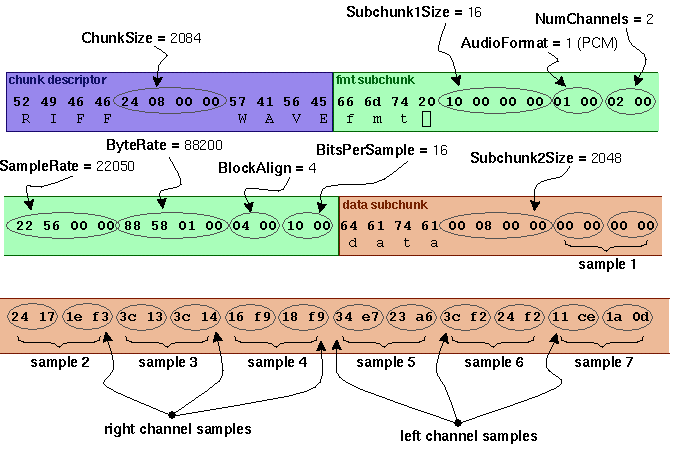
\includegraphics[scale=0.65]{attēli/wave-bytes.png}
     \caption{WAV faila struktūra. \parencite{wav_struktura}}
    \label{fig:wavebytes}
    
\end{figure}
    \\Izmantojot C programmēšanas valodas faila ielādes funkcijas, šis WAV fails tiek ielasīts un sadalīts daļās pa 8 bitiem. Atsevišķos masīvos tiek ielasīti WAV faila baiti, kā veseli \emph{int} skaitļi, un katrs pirmais bits, nultajā indeksā, no katras 8 bitu, jeb 1 baita virknes, jo katrs paraugs arī tiek kodēts \emph{little-endian} formātā, un pirmais bits arī tajā ir vismazsvarīgākais, jeb vismainīgākais, t.i. 8 bitu veselam skaitlim robežās no 0 līdz 255 tas atbild par vieniem un izmaina tikai par vērtību 1. Tālāk C iekļauto bibliotēku limitāciju dēļ šie biti, kas saglabāti kā veseli skaitļi, tiek ierakstīti kā binārā heksadecimālā formātā, kā \emph{.bin} fails. Testēšanas programmatūrā tiks testēti tikai šie faili, jo atbilst to nepieciešamajam binārajam faila formātam. Visa 8 bitu, jeb 1 baita virkne tiek ielasīta masīvā, kā veseli skaitļi (0 vai 1), kuru izmanto funkcijā, kas paņem izvēlēto robežu starpību: 
    \[
    \log_2 (max - min)
    \]
    un izveido decimālus veselos skaitļus, ņemot šīs starpības bitu skaitu, kas apaļots uz augšu. Ja izveidotais skaitlis neietilpst noteiktajās robežās, tas netiek ielasīts, bet, ja ietilpst, tas tiek saglabāts atsevišķā failā, kurā ieraksta izveidotos failus \emph{ASCII} formātā.  
    
    \subsection{Datu ieguves veikšana}
    
    Dati tiek ievākti ierakstot atmosfērisko troksni audio formātā dažādās radio frekvencēs, kas ietilpst \emph{FM} un \emph{AM} radio frekvenču diapazonos, un apstrādājot tos caur izveidoto programmu. Atmosfēriskā radio trokšņa ierakstīšana norisinās, izmantojot USB audiosaskarsni, kas savienota ar portatīva radio aparāta audio izeju. Radio frekvences tika izvēlētas pēc tajās pārraidīto radio staciju radītā trokšņa daudzuma, izvēloties frekvences ar pēc iespējas mazāku radio staciju radīto troksni; pārsvarā tiek testētas frekvences, kas ietilpst \emph{AM} frekvenču diapazonā,limitēto radio frekvenču robežu dēļ. Ievadot audio failus izveidotajā programmā, tiek iegūti 2 faili:
    \emph{108MHz\_biti.txt} un 
    \emph{108MHz\_biti\_robezas.txt}, kas ir ASCII formātā, un \emph{108MHz\_mazsvarigakie\_biti.bin}, kas ir binārais fails un tiks ievadīts
    nejaušuma testēšanas programmā. Fails \emph{108MHz\_biti.bin} NIST SP-800 22 nejaušuma tiek ievadīts testēšanas programmā,
    izsaucot sākotnējo testkomplekta konsoles izpildāmo failu \emph{./assess} ar argumentu \emph{bitu\_plūsmas\_garums}, kas tiek aprēķināts pēc formulas:
    \[
    \text{bitu plūsmas garums} = \frac{\text{kopējais faila lielums bitos}}{\text{bitu plūsmu skaits}}
    \]
    bitu plūsmu skaits norāda uz skaitli, cik daļās ar izmēru \emph{bitu\_plūsmas\_garums} tiks sadalīts viss fails. Lai atvieglotu testa rezultātu analīzi, bitu plūsmu skaits tiek iestatīts uz 100. 
    Tālāk testēšanas programmā tiek atlasīta opcija 0, lai ievadītu ārēju failu, un tiek piemēroti visi statistikas testi, bitu plūsmu skaits tiek iestatīts uz 100. Apskatāmi testkomplekta rezultāti \textbf{\ref{rezultati_108} tabulā}.
    %(Vajag vairāk nbet nekā)   
    \section{Rezultāti un to analīze}
    Rezultātu analīze ir strukturēta 6 daļās. Ir aplūkoti un testēti dati, kas ģenerēti, izmantojot 520, 620, 660 kHz, 1500 kHz un 108 MHz frekvencēs ierakstīto radio troksni, kā arī analizēti kontroles dati, ko ģenerējis pseido-nejaušu skaitļu ģenerators. Šajās daļās ir aplūkota statistiskā nejaušuma analīze iegūtajiem datiem, izmantojot \emph{NIST} SP 800-22 testkomplektu. Ir izteikta augstākās nejaušības, jeb entropijas kvalitātes frekvence, un veidoti secinājumi par datu nejaušumu atkarībā no testēto frekvenču augstuma. 
    
    \subsection{Nejašuma tests 108 MHz frekvencē}
    Ierakstot atmosfērisko radio troksni 108 MHz frekvencē audio formātā, ievadot to izveidotajā programmā un iegūtos datus ievadot NIST SP-800 statistiskajā testkomplektā nejaušiem un pseido nejaušiem skaitļiem, iegūst rezultātu vērtības dažādos statistiskajos pārbaudījumos datu nejaušuma testēšanai. Dati ir apkopoti un sakārtoti \textbf{\ref{rezultati_108} tabulā}.

\begin{table}[!ht]
\centering


\begin{tabular}{ |c|c|c| }% c automātiski padara kolonnu tik garu cik vajag
\hline
Statistiskais pārbaudījums & Proporcija & P-vērtība \\
\hline
Biežuma (monobitu) & 0/100 & 0,000000\\
\hline
Nepārklājošie Paraugi & 99/100 & 0,554420 \\
\hline
Lineārā sarežģītība & 98/100 & 0,289667 \\
\hline
\end{tabular}

\caption{108 MHz frekvences datu nejaušuma statistiskie rezultāti \\ \emph{NIST SP 800-22 testkomplektā}.\parencite{NIST_orig}}

\label{rezultati_108}
\end{table}

  \FloatBarrier
    
    Aplūkojot iegūtos rezultātus, var novērot, ka  biežuma, jeb monobitu pārbaudījumā neviena no 100 bitu plūsmām neizpildīja nosacījumu, ka nullēm un vieniniekiem ir jābūt aptuveni vienādi sadalītiem, bet ņemot vērā, ka ģenerēto skaitļu avots ir atmosfēriskais radio troksnis un šis process skaidrojams kā nejaušs, sadalījums var nebūt aptuveni vienāds. Nepārklājošo paraugu pārbaudījumā ir vislielākā P-vērtība no visiem izmantotajiem statistiskajiem testiem un tā norāda uz ģenerēto skaitļu aperiodiskumu un nenoteiktību. Novērojams datu nejaušums attiecībā uz šo kritēriju, kaut arī P-vērtība norāda, ka varbūtība, ka šī nepārklājošo paraugu hipotēze izpildās, ir tikai aptuveni 55,4\%, kaut gan jebkura P-vērtība, kas lielāka par 0, norāda uz to, ka dati ir nejauši.
    Lineārās sarežģītības pārbaudījuma P-vērtība, savukārt, norāda, ka aprēķinātais lineāras atsauces nobīdes reģistra garums ir salīdzinoši īss un tāpēc sarežģītība šai virknei nav augsta.

%%%%%%%%%%%%%%%%%%%%%%%%%%%%%%%
    \subsection{Nejašuma tests 1500 kHz frekvencē}
    Ierakstot atmosfērisko radio troksni 1500 kHz frekvencē audio formātā, ievadot to izveidotajā programmā un iegūtos datus ievadot NIST SP-800 statistiskajā testkomplektā nejaušiem un pseido nejaušiem skaitļiem, iegūst rezultātu vērtības dažādos statistiskajos pārbaudījumos datu nejaušuma testēšanai. Dati ir apkopoti un sakārtoti \textbf{\ref{rezultati_1500} tabulā}.

\begin{table}[!ht]
\centering


\begin{tabular}{ |c|c|c| }% c automātiski padara kolonnu tik garu cik vajag
\hline
Statistiskais pārbaudījums & Proporcija & P-vērtība \\
\hline
Biežuma (monobitu) & 41/100 & 0,000000\\
\hline
Nepārklājošie Paraugi & 100/100 & 0,153763 \\
\hline
Lineārā sarežģītība & 99/100 & 0,455937 \\
\hline
\end{tabular}

\caption{1500 kHz frekvences datu nejaušuma statistiskie rezultāti \\ \emph{NIST SP 800-22 testkomplektā}.\parencite{NIST_orig}}

\label{rezultati_1500}
\end{table}

  \FloatBarrier  
    
    Aplūkojot iegūtos rezultātus, var novērot, ka  biežuma, jeb monobitu pārbaudījumā 41 no 100 bitu plūsmām izpildīja nosacījumu, ka nullēm un vieniniekiem ir jābūt aptuveni vienādi sadalītiem, bet P-vērtība ir 0, tas var liecināt par to, ka kādā brīdī, kad tika ierakstīti dati, bija radio traucējums, kas atlikušos datus darīja nepilnīgus, jo P-vērtībai būtu jāatspoguļo šo 41 bitu plūsmu šī pārbaudījuma izpildīšanu, bet ņemot vērā, ka ģenerēto skaitļu avots ir atmosfēriskais radio troksnis, pastāv iespējama iejaukšanās radio signālā no mākslīgiem avotiem. Nepārklājošo paraugu pārbaudījumā P-vērtība, savukārt, no visiem izmantotajiem statistiskajiem testiem un tā norāda uz ģenerēto skaitļu aperiodiskumu un nenoteiktību. Novērojams datu nejaušums attiecībā uz šo kritēriju, kaut arī P-vērtība norāda, ka varbūtība, ka šī nepārklājošo paraugu hipotēze izpildās, ir tikai aptuveni 15,4\%, kaut gan jebkura P-vērtība, kas lielāka par 0 liecina par datu nejaušumu.
    Lineārās sarežģītības pārbaudījuma P-vērtība, savukārt, norāda, ka aprēķinātais lineāras atsauces nobīdes reģistra garums ir salīdzinoši garš un tāpēc sarežģītība šai virknei ir uzskatāma par diezgan augstu.

%%%%%%%%%%%%%%%%%%%%%%%%%%%

\subsection{Nejašuma tests 660 kHZ frekvencē}

    Ierakstot atmosfērisko radio troksni 660 kHz frekvencē audio formātā, ievadot to izveidotajā programmā un iegūtos datus ievadot NIST SP-800 statistiskajā testkomplektā nejaušiem un pseido nejaušiem skaitļiem, iegūst rezultātu vērtības dažādos statistiskajos pārbaudījumos datu nejaušuma testēšanai. Dati ir apkopoti un sakārtoti \textbf{\ref{rezultati_660} tabulā}.

\begin{table}[!ht]
\centering


\begin{tabular}{ |c|c|c| }% c automātiski padara kolonnu tik garu cik vajag
\hline
Statistiskais pārbaudījums & Proporcija & P-vērtība \\
\hline
Biežuma (monobitu) & 0/100 & 0,000000\\
\hline
Nepārklājošie Paraugi & 98/100 & 0,678686 \\
\hline
Lineārā sarežģītība & 99/100 & 0,616305 \\
\hline
\end{tabular}

\caption{660 kHz frekvences datu nejaušuma statistiskie rezultāti \\ \emph{NIST SP 800-22 testkomplektā}.\parencite{NIST_orig}}

\label{rezultati_660}
\end{table}

  \FloatBarrier
    Aplūkojot iegūtos rezultātus, var novērot, ka  biežuma, jeb monobitu pārbaudījumā neviena no 100 bitu plūsmām neizpildīja nosacījumu, ka nullēm un vieniniekiem ir jābūt aptuveni vienādi sadalītiem, bet ņemot vērā, ka ģenerēto skaitļu avots ir atmosfēriskais radio troksnis un šis process skaidrojams kā nejaušs, sadalījums var nebūt aptuveni vienāds. Nepārklājošo paraugu pārbaudījumā ir vislielākā P-vērtība no visiem izmantotajiem statistiskajiem testiem un tā norāda uz ģenerēto skaitļu aperiodiskumu un nenoteiktību. Novērojams datu nejaušums attiecībā uz šo kritēriju, P-vērtība virs 0,65 norāda uz gandrīz noteiktu aperiodiskumu, kaut gan jebkura P-vērtība, kas lielāka par 0 norāda uz to, ka dati ir nejauši, vērtība virs 0,5 izrāda īpaši augstu nejaušumu un entropiju.
    Lineārās sarežģītības pārbaudījuma P-vērtība virs 0,6, savukārt, norāda, ka aprēķinātais lineāras atsauces nobīdes reģistra garums ir garš un tāpēc sarežģītība šai virknei ir uzskatāma par ļoti augstu un šis nejaušuma tests arī noteikti izpildās.

%%%%%%%%%%%%%%
    \subsection{Nejašuma tests 620kHZ frekvencē}

    Ierakstot atmosfērisko radio troksni 620 kHz frekvencē audio formātā, ievadot to izveidotajā programmā un iegūtos datus ievadot NIST SP-800 statistiskajā testkomplektā nejaušiem un pseido nejaušiem skaitļiem, iegūst rezultātu vērtības dažādos statistiskajos pārbaudījumos datu nejaušuma testēšanai. Dati ir apkopoti un sakārtoti \textbf{\ref{rezultati_620} tabulā}.

\begin{table}[!ht]
\centering


\begin{tabular}{ |c|c|c| }% c automātiski padara kolonnu tik garu cik vajag
\hline
Statistiskais pārbaudījums & Proporcija & P-vērtība \\
\hline
Biežuma (monobitu) & 0/100 & 0,000000\\
\hline
FFT & 0/100 & 0,000000\\
\hline
Nepārklājošie Paraugi & 97/100 & 0,455937 \\ %0,181557
\hline
Lineārā sarežģītība & 98/100 & 0,007160 \\
\hline
\end{tabular}

\caption{620 kHz frekvences datu nejaušuma statistiskie rezultāti \\ \emph{NIST SP 800-22 testkomplektā}.\parencite{NIST_orig}}

\label{rezultati_620}
\end{table}
\FloatBarrier
    Aplūkojot iegūtos rezultātus, var novērot, ka  biežuma, jeb monobitu pārbaudījumā neviena no 100 bitu plūsmām neizpildīja nosacījumu, ka nullēm un vieniniekiem ir jābūt aptuveni vienādi sadalītiem, bet ņemot vērā, ka ģenerēto skaitļu avots ir atmosfēriskais radio troksnis un šis process skaidrojams kā nejaušs, sadalījums var nebūt aptuveni vienāds. Nepārklājošo paraugu pārbaudījumā ir vislielākā P-vērtība no visiem izmantotajiem statistiskajiem testiem un tā norāda uz ģenerēto skaitļu aperiodiskumu un nenoteiktību. Novērojams datu nejaušums attiecībā uz šo kritēriju, arī P-vērtība norāda, ka varbūtība, ka šī nepārklājošo paraugu hipotēze izpildās, ir vidēja, jo P-vertība ir aptuveni 45,5\% 
    Lineārās sarežģītības pārbaudījuma P-vērtība, savukārt, norāda, ka aprēķinātais lineāras atsauces nobīdes reģistra garums ir ļoti īss un tāpēc sarežģītība šai virknei nav augsta un nejaušums tātad arī, jo P-vērtība ir tikai aptuveni 0,07\%.



%%%%%%%%%%%%%%%%%%%%%%%%%%5
    \subsection{Nejašuma tests 520 kHZ frekvencē}

    Ierakstot atmosfērisko radio troksni 520 kHz frekvencē audio formātā, ievadot to izveidotajā programmā un iegūtos datus ievadot NIST SP-800 statistiskajā testkomplektā nejaušiem un pseido nejaušiem skaitļiem, iegūst rezultātu vērtības dažādos statistiskajos pārbaudījumos datu nejaušuma testēšanai. Dati ir apkopoti un sakārtoti \textbf{\ref{rezultati_520} tabulā}.

\begin{table}[!ht]
\centering

\begin{tabular}{ |c|c|c| }% c automātiski padara kolonnu tik garu cik vajag
\hline
Statistiskais pārbaudījums & Proporcija & P-vērtība \\
\hline
Biežuma (monobitu) & 0/100 & 0,000000\\
\hline
Nepārklājošie Paraugi & 94/100 & 0,045675 \\
\hline
Lineārā sarežģītība & 98/100 & 0,171867 \\
\hline
\end{tabular}

\caption{520 kHz frekvences datu nejaušuma statistiskie rezultāti \\ \emph{NIST SP 800-22 testkomplektā}.\parencite{NIST_orig}}

\label{rezultati_520}
\end{table}

  \FloatBarrier
    Aplūkojot iegūtos rezultātus, var novērot, ka  biežuma, jeb monobitu pārbaudījumā neviena no 100 bitu plūsmām neizpildīja nosacījumu, ka nullēm un vieniniekiem ir jābūt aptuveni vienādi sadalītiem. Nepārklājošo paraugu pārbaudījumā , kas norāda uz ģenerēto skaitļu aperiodiskumu un nenoteiktību, novērojams datu nejaušums attiecībā uz šo kritēriju, kaut gan varbūtība, ka šī nepārklājošo paraugu hipotēze izpildās, ir tikai aptuveni 4,5\%, bet jebkura P-vērtība, kas lielāka par 0 norāda uz to, ka dati ir nejauši.
    Lineārās sarežģītības pārbaudījuma P-vērtība, savukārt, norāda, ka aprēķinātais lineāras atsauces nobīdes reģistra garums ir salīdzinoši īss un tāpēc sarežģītība šai virknei nav augsta, varbūtība, ka tā izpildās ir tikai 17,1\%. 

    
%%%%%%%%%%%%%%%%%%%%%%%%%%%%
 \subsection{Nejašuma tests XOR pseido-nejaušu skaitļu ģeneratoram}

    NIST SP-800 statistiskajā testkomplektā nejaušiem un pseido nejaušiem skaitļiem tiek ievadīta izvēle testēt datus, kas ģenerēti ar XOR nobīdes (Xorshift) pseido-nejaušu skaitļu ģeneratoru, kas ir viens no ātrākajiem pseido-nejaušu skaitļu ģeneratoriem. Dati ir apkopoti un sakārtoti \textbf{\ref{rezultati_xor} tabulā}.

\begin{table}[!ht]
\centering

\begin{tabular}{ |c|c|c| }% c automātiski padara kolonnu tik garu cik vajag
\hline
Statistiskais pārbaudījums & Proporcija & P-vērtība \\
\hline
Biežuma (monobitu) & 62/100 & 0,000000\\
\hline
Nepārklājošie Paraugi & 50/100 & 0,000000 \\
\hline
Lineārā sarežģītība & 0/100 & 0,000000 \\
\hline
\end{tabular}

\caption{Xorshift ģeneratora datu nejaušuma statistiskie rezultāti \\ \emph{NIST SP 800-22 testkomplektā}.\parencite{NIST_orig}}

\label{rezultati_xor}
\end{table}

  \FloatBarrier
     Aplūkojot iegūtos rezultātus, var novērot, ka biežuma, jeb monobitu pārbaudījumā 62 no 100 bitu plūsmām izpildīja nosacījumu, ka nullēm un vieniniekiem ir jābūt aptuveni vienādi sadalītiem, bet P-vērtība ir 0, kas nozīmē to, ka nulles un vieninieki ir ļoti neproporcionāli sadalīti. Nepārklājošo paraugu pārbaudījumā P-vērtība, savukārt, ir arī 0, bet 50 no 100 bitu plūsmām ir izpildījušas testu, kas norāda uz vairākkārtēju paraugu atkārtošanos.
    Lineārās sarežģītības pārbaudījuma P-vērtība, savukārt, norāda, ka aprēķinātais lineāras atsauces nobīdes reģistra garums ir ļoti īss un tāpēc sarežģītība šai virknei ir uzskatāma par ļoti mazu. Šī ģeneratora datus noteikti nevar uzskatīt par nejaušiem.


    
    \subsection{Kopsavilkuma analīze}
    Starp radio frekvencēm, kurās ierakstīts atmosfēriskais radio troksnis, var saskatīt ļoti lielu dažādību tā ģenerēto skaitļu nejaušumā. Visnekvalitatīvākās frekvences, kurās ierakstīts atmosfēriskais radio troksnis, ir 520 kHz un 620 kHz, savukārt kvalitatīvākā ir 660 kHz. Var secināt, ka tas varētu būt skaidrojums ar radio staciju blīvo AM un FM radio diapazonu nosegumu, kā arī no mākslīgiem avotiem radīto elektromagnētisko viļņu iejaukšanos un signāla slāpēšanu. Pseido-nejaušu skaitļu ģeneratora kontroles nejaušuma pārbaude pierāda pseido-nejaušo skaitļu ģeneratoru mazo uzticamību un nepilnības skaitļu neparedzamībā. Pētījumā izmantoto atmosfēriskā radio trokšņa ieguves radio frekvences visas ietilpst AM un FM diapazonos (535-1605 kHz un 88-108 MHz), jo tie ir vienīgie, kas viegli pieejami ar jebkuru radioaparātu, bet ir, galvenokārt, paredzēti radio staciju pārraidēm un slāpē atmosfērisko radio troksni arī blakus frekvencēs, pat ja netiek pārraidīti tieši tajā, novedot pie nekvalitatīva atmosfēriskā radio trokšņa signāla un neapstiprināmu nejaušumu no tā ģenerētajām skaitļu virknēm, ko pierāda statistiskie pārbaudījumi. 
    \par
    Turpmākajos pētījumos būtu iespējams izmantot citas radio frekvences, kas ir ārpus šiem AM un FM diapazoniem, kurās nepastāv blīvs pārklājums ar mākslīgu avotu radītiem radio signāļiem, izmantojot specializētas radio antennas ar atsevišķu uztvērēju, lai iegūtu augstas kvalitātes atmosfēriskā trokšņa radio signālu ar maksimāli minimālām aŗējiem traucēkļiem. Kā arī izveidot ilgtermiņa risinājumu, kas nepārtraukti no uztvertā atmosfēriskā radio trokšņā ģenerē pilnīgi nejaušus skaitļus, lai padarītu tos vēl pieejamākus ikvienai izmantošanas nozīmei.

    \pagebreak
    \section{Secinājumi}
    \begin{enumerate}
        \item Pētijumā piedāvātais īsti nejaušu skaitļu ģenerators statistiskajos pārbaudījumos uzstāda labākus rezultātus par bieži izmantoto Xorshift pseido-nejaušo skaitļu ģeneratoru.
        \item Pilnīgi nejauši skaitļu ģeneratori ir daudz uzticamāki un statistiski entropijā bagātāki par pseido-nejaušu skaitļu ģeneratoriem.
        \item Balstoties uz pētijumu, iespējams mājās apstākļos iegūt pilnīgi nejaušus skaitļus no atmosfēriskā radio trokšņa.
        \item Izmantojot radio frekvences, kurās iespējama makslīgo radio signālu iejaukšanās, ģenerēto skaitļu virkņu statistiskā nejaušuma kvalitāte būtiski samazinās.
    \end{enumerate}
    
    %atsauces
    \pagebreak
    %\section{Literatūras apskats}
    %\bibliographystyle{apalike}
    %\bibliography{bibliografija}
    \fakesection{Literatūras saraksts}
    
    \printbibliography
    \pagebreak
\komentars{
    \section{Pielikumi}
    \appendix
    \begin{figure}[!ht]
    \raggedleft \caption{Caption}
    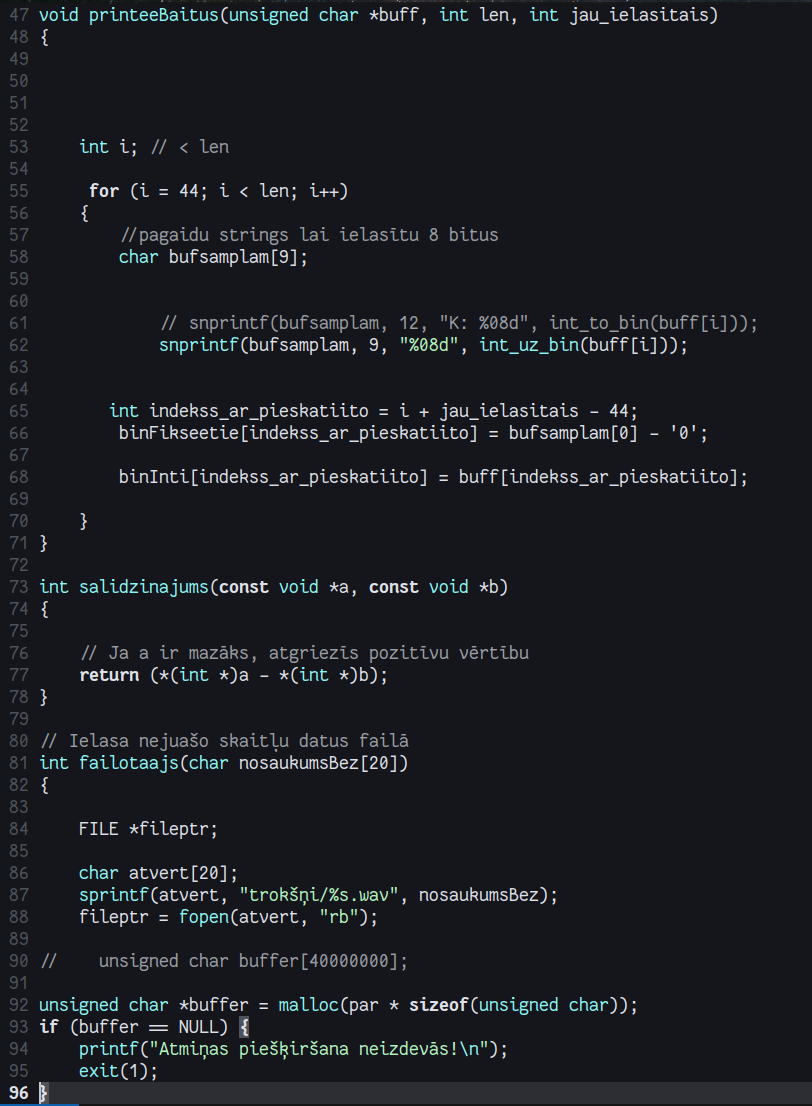
\includegraphics{attēli/Attēli_1.png}
    
\end{figure}
\begin{figure}[!ht]
    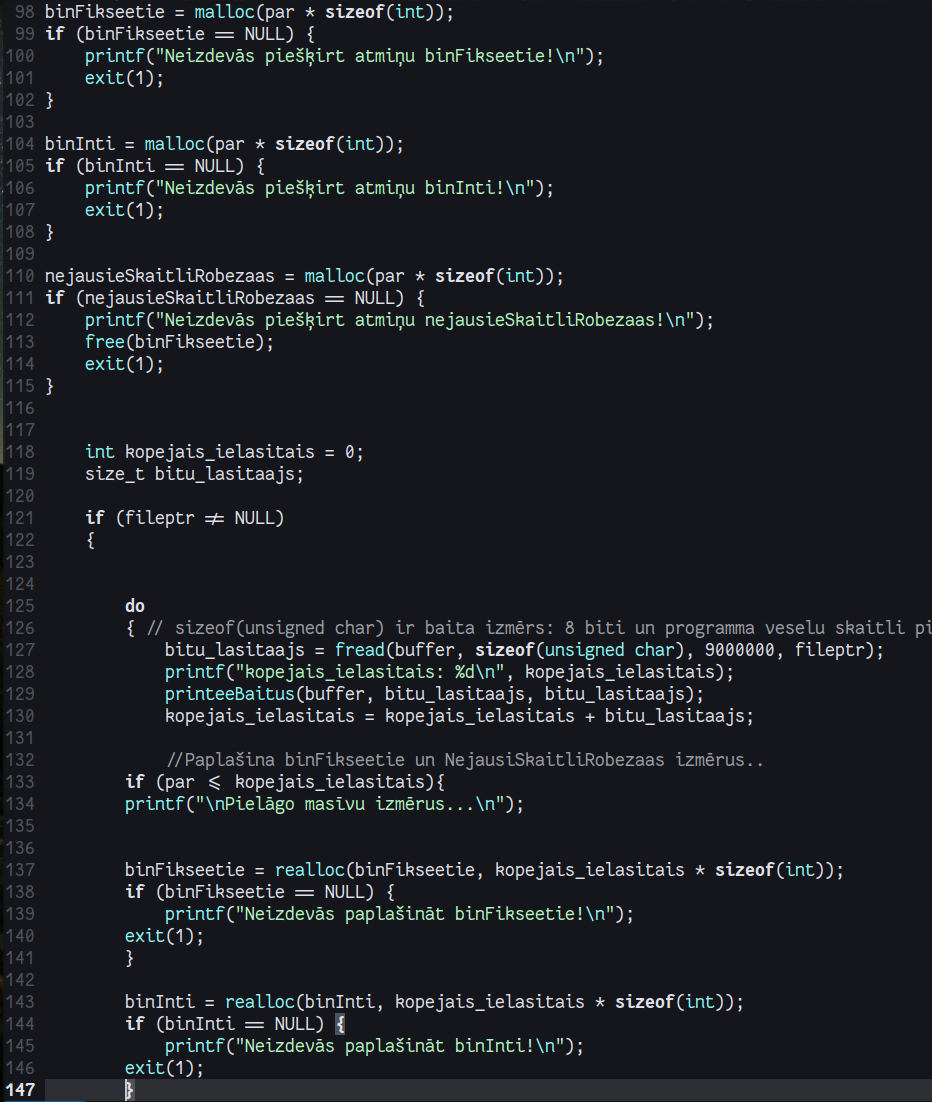
\includegraphics{attēli/Attēli_2.png}
\end{figure}[!ht]
\begin{figure}
    \centering
    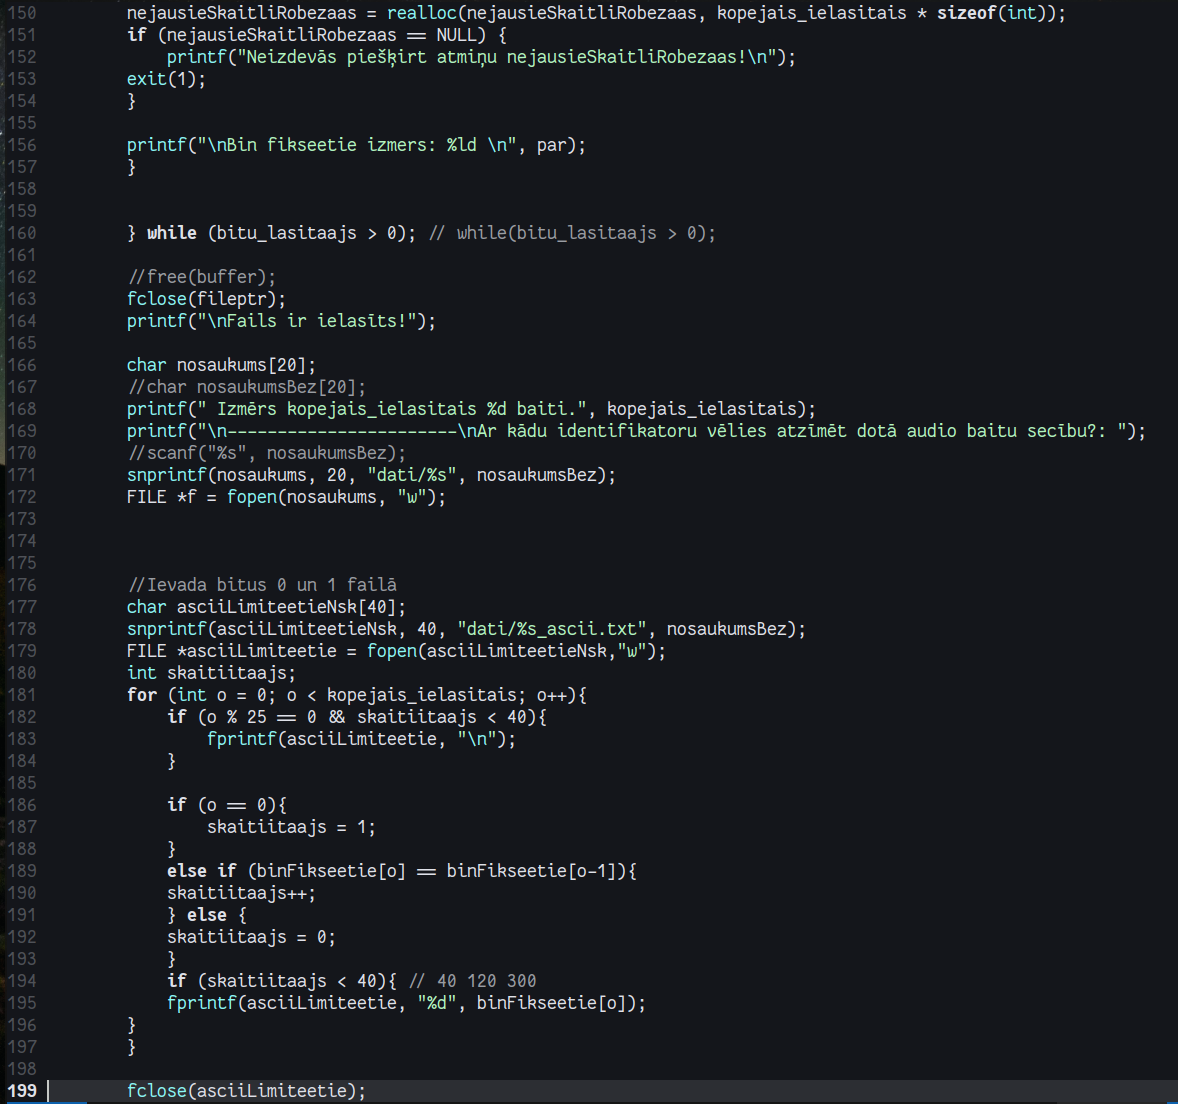
\includegraphics{attēli/Attēli_3.png}
\end{figure}

\begin{figure}[!ht]
    \centering
    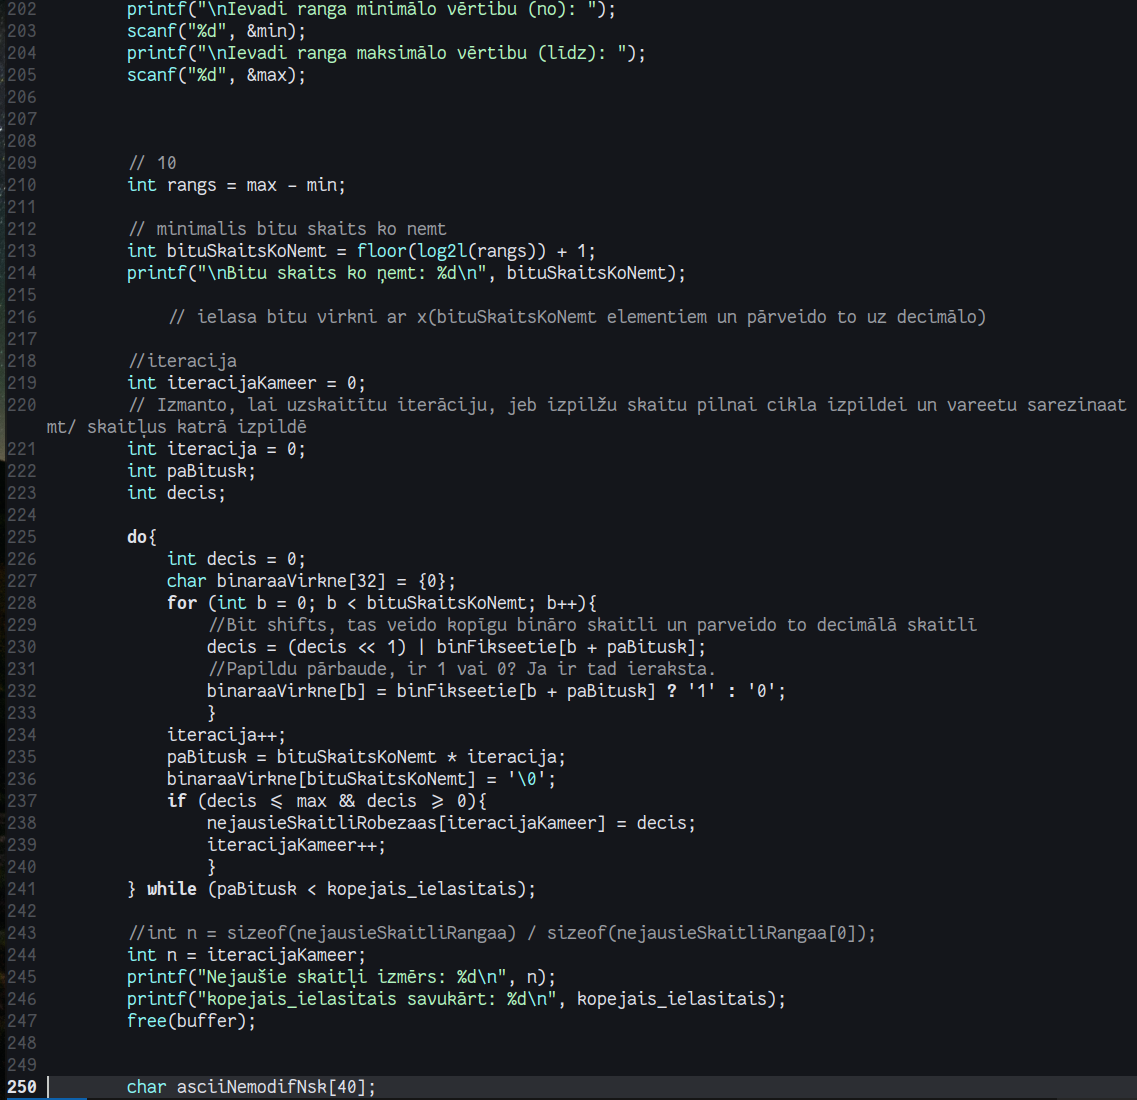
\includegraphics{attēli/Attēli_4.png}
\end{figure}

\begin{figure}[!ht]
    \centering
    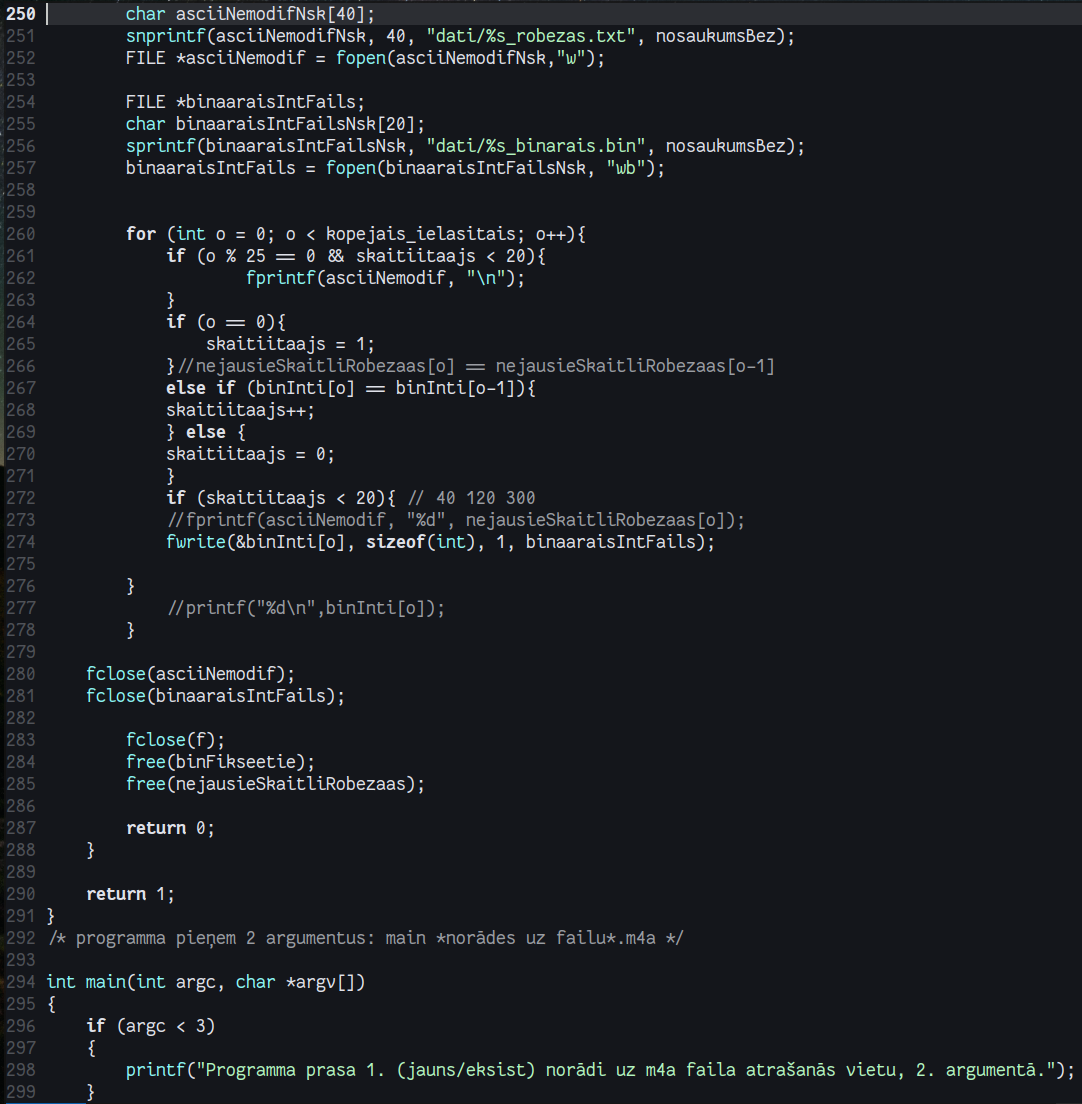
\includegraphics{attēli/Attēli_5.png}
\end{figure}

\begin{figure}[!ht]
    \centering
    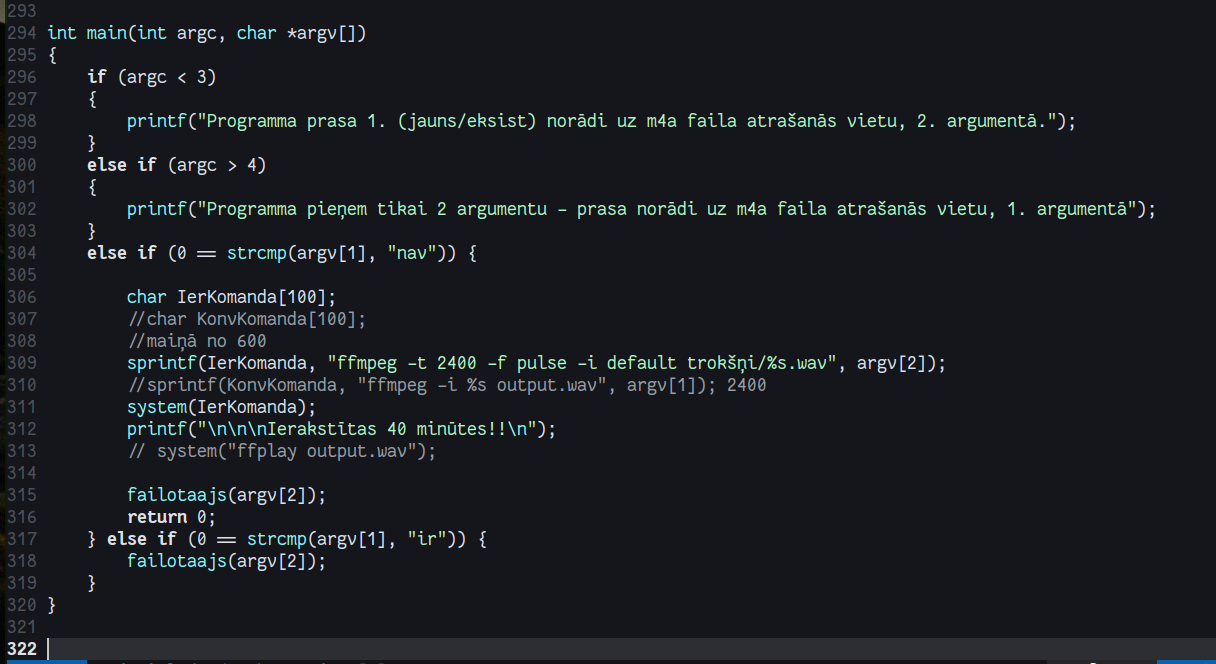
\includegraphics{attēli/Attēli_6.png}
\end{figure}
}

\end{document}
